%% The first command in your LaTeX source must be the \documentclass command.
\documentclass[sigconf]{acmart}
%% NOTE that a single column version is required for 
%% submission and peer review. This can be done by changing
%% the \doucmentclass[...]{acmart} in this template to 
%% \documentclass[manuscript,screen]{acmart}
%% 
%% To ensure 100% compatibility, please check the white list of
%% approved LaTeX packages to be used with the Master Article Template at
%% https://www.acm.org/publications/taps/whitelist-of-latex-packages 
%% before creating your document. The white list page provides 
%% information on how to submit additional LaTeX packages for 
%% review and adoption.
%% Fonts used in the template cannot be substituted; margin 
%% adjustments are not allowed.

%%
%% \BibTeX command to typeset BibTeX logo in the docs
\AtBeginDocument{%
  \providecommand\BibTeX{{%
    \normalfont B\kern-0.5em{\scshape i\kern-0.25em b}\kern-0.8em\TeX}}}

%% Add images folder as source for graphics
\graphicspath{ {images/} }

%% Library to draw ERD diagrams
\usepackage{array}
\renewcommand{\arraystretch}{1.1}
\usepackage{tikz}
\usetikzlibrary{shapes.multipart}
\usetikzlibrary{positioning}
\usetikzlibrary{shadows}
\usetikzlibrary{calc}

\usepackage{pdflscape}

% code for "one to omany", etc. is taken from https://tex.stackexchange.com/q/141797/101651
\makeatletter
\pgfarrowsdeclare{crow's foot}{crow's foot}
{
    \pgfarrowsleftextend{+-.5\pgflinewidth}%
    \pgfarrowsrightextend{+.5\pgflinewidth}%
}
{
    \pgfutil@tempdima=0.6pt%
    \pgfsetdash{}{+0pt}%
    \pgfsetmiterjoin%
    \pgfpathmoveto{\pgfqpoint{0pt}{-9\pgfutil@tempdima}}%
    \pgfpathlineto{\pgfqpoint{-13\pgfutil@tempdima}{0pt}}%
    \pgfpathlineto{\pgfqpoint{0pt}{9\pgfutil@tempdima}}%
    \pgfpathmoveto{\pgfqpoint{0\pgfutil@tempdima}{0\pgfutil@tempdima}}%
    \pgfpathmoveto{\pgfqpoint{-8pt}{-6pt}}% 
    \pgfpathlineto{\pgfqpoint{-8pt}{-6pt}}%  
    \pgfpathlineto{\pgfqpoint{-8pt}{6pt}}% 
    \pgfusepathqstroke%
}

\pgfarrowsdeclare{omany}{omany}
{
    \pgfarrowsleftextend{+-.5\pgflinewidth}%
    \pgfarrowsrightextend{+.5\pgflinewidth}%
}
{
    \pgfutil@tempdima=0.6pt%
    \pgfsetdash{}{+0pt}%
    \pgfsetmiterjoin%
    \pgfpathmoveto{\pgfqpoint{0pt}{-9\pgfutil@tempdima}}%
    \pgfpathlineto{\pgfqpoint{-13\pgfutil@tempdima}{0pt}}%
    \pgfpathlineto{\pgfqpoint{0pt}{9\pgfutil@tempdima}}%
    \pgfpathmoveto{\pgfqpoint{0\pgfutil@tempdima}{0\pgfutil@tempdima}}%  
    \pgfpathmoveto{\pgfqpoint{0\pgfutil@tempdima}{0\pgfutil@tempdima}}%
    \pgfpathmoveto{\pgfqpoint{-6pt}{-6pt}}% 
    \pgfpathcircle{\pgfpoint{-11.5pt}{0}} {3.5pt}
    \pgfusepathqstroke%
}

\pgfarrowsdeclare{one}{one}
{
    \pgfarrowsleftextend{+-.5\pgflinewidth}%
    \pgfarrowsrightextend{+.5\pgflinewidth}%
}
{
    \pgfutil@tempdima=0.6pt%
    \pgfsetdash{}{+0pt}%
    \pgfsetmiterjoin%
    \pgfpathmoveto{\pgfqpoint{0\pgfutil@tempdima}{0\pgfutil@tempdima}}%
    \pgfpathmoveto{\pgfqpoint{-6pt}{-6pt}}% 
    \pgfpathlineto{\pgfqpoint{-6pt}{-6pt}}%  
    \pgfpathlineto{\pgfqpoint{-6pt}{6pt}}% 
    \pgfpathmoveto{\pgfqpoint{0\pgfutil@tempdima}{0\pgfutil@tempdima}}%
    \pgfpathmoveto{\pgfqpoint{-8pt}{-6pt}}% 
    \pgfpathlineto{\pgfqpoint{-8pt}{-6pt}}%  
    \pgfpathlineto{\pgfqpoint{-8pt}{6pt}}%    
    \pgfusepathqstroke%
}
\makeatother

\tikzset{%
    pics/entity/.style n args={3}{code={%
        \node[draw,
        rectangle split,
        rectangle split parts=2,
        text height=1.5ex,
        ] (#1)
        {#2 \nodepart{second}
            \begin{tabular}{>{\raggedright\arraybackslash}p{8.5em}}
                #3
            \end{tabular}
        };%
    }},
    pics/entitynoatt/.style n args={2}{code={%
        \node[draw,
        text height=1.5ex,
        ] (#1)
        {#2};%
    }},
    zig zag to/.style={
        to path={(\tikztostart) -| ($(\tikztostart)!#1!(\tikztotarget)$) |- (\tikztotarget)}
    },
    zig zag to/.default=0.5,   
    one to one/.style={
        one-one, zig zag to
    },
    one to oone/.style={            % I do not how to make "one to Optional-one" rel
        one-one, zig zag to
    },
    one to many/.style={
        one-crow's foot, zig zag to,
    },
    one to omany/.style={
        one-omany, zig zag to
    }
}

%% Begin document
\begin{document}


%% The "title" command has an optional parameter,
%% allowing the author to define a "short title" to be used in page headers.
\title{Master Thesis Proposal: Risk detection and risk control through sprint backlog analysis}

%%
%% The "author" command and its associated commands are used to define
%% the authors and their affiliations.
%% Of note is the shared affiliation of the first two authors, and the
%% "authornote" and "authornotemark" commands
%% used to denote shared contribution to the research.
\author{Sytse Groenwold}
\affiliation{13083228}
\email{sytse.groenwold@student.uva.nl}

\author{Zhiming Zhao}
\affiliation{Supervisor}
\email{z.zhao@uva.nl}

\author{TBD}
\affiliation{Examiner}
\email{email}

%%
%% By default, the full list of authors will be used in the page
%% headers. Often, this list is too long, and will overlap
%% other information printed in the page headers. This command allows
%% the author to define a more concise list
%% of authors' names for this purpose.
\renewcommand{\shortauthors}{Groenwold, S.}

%%
%% The abstract is a short summary of the work to be presented in the
%% article.
\begin{abstract}

Abstract comes here in the final stage of writing. \\

\end{abstract}

%%
%% Keywords. The author(s) should pick words that accurately describe
%% the work being presented. Separate the keywords with commas.
\keywords{Keywords come here in the final stage of writing.}

%%
%% This command processes the author and affiliation and title
%% information and builds the first part of the formatted document.
\maketitle

\section{Introduction}
In software development, there are several risk events that can decrease product quality, delay delivery or even cause the project to fail[2]. 
Tangible examples of these events are budget overruns and losing personnel, while more subtle ones include a lack of clearly defining work to be done or team members being unaligned. 
(Early) detection (i.e. risk assessment) of such risks and controlling them effectively (i.e. risk control) is crucial for the success of a project[3].

The Agile development methodologies have demonstrated their advantages over traditional methods in reducing time to market, overall product quality and a closer alignment to business needs[5]. 
In Scrum, this is achieved through an iterative process over a short period of time; these iterations are called sprints.
The product manager creates a backlog of user stories, which are the business requirements translated into pieces work for the development team. 
During a sprint, the team works on a selected number of these user stories and afterwards they reflect on both the work done and the collaboration within the team.
Despite these improved practices, Agile methodologies can still suffer from risks: unclear user stories, inefficient decomposition, and scheduling of the sprint backlogs. 
Determining those risk through analysis of the user stories in the product backlog is mostly done by human experts. 

In a previous study, we sought to automate this process, by creating an machine learning model based on previous works and ensembling those models. 

While those results show promise for a machine learning model to detect risks, improvement is needed to make the predictions more robust, especially to achieve more consistent scores between different datasets.
We determined that incorporating the sprint plannings, instead of only analysing the individual user stories, could be a valuable addition to the model parameters in achieving this goal. In this study we plan to do that, and additionally investigate a way to single-out the specific risks that are inside a sprint backlog, so that teams can exercise risk control before they affect the team output.

Among the different software packages used by Scrum adaptors to track user stories, Jira is by far the most used one, having a large margin over other comparable services, according to slintel\footnote{https://www.slintel.com/tech/bug-and-issue-tracking/atlassian-jira-market-share}, Datalyze\footnote{https://www.datanyze.com/market-share/project-management--217/jira-market-share}, and Enlyft\footnote{https://enlyft.com/tech/products/atlassian-jira}. It is however still under represented in software engineering research, according to Montgomery et al.\cite{montgomery2022jira}; for this reason they published their dataset with the most extensive collection of publicly available Jira repositories to date.

\subsection{Research question}
\textbf{Q1}. To what extent can the inclusion of sprint backlog in issue analysis improve risk assessment within software teams using Scrum and \textbf{Q2}. which features of such a model are most impactful risk assessment and risk control?

\subsection{Sub questions}
The sub questions are:

\textbf{Q1.1}: How many publicly available Jira repositories have their sprint data available?

\textbf{Q1.2}: Is it possible to include this data as a single feature into existing models, or would a separate model added to the ensembling method perform better?

\textbf{Q2.1}: Is the sprint data a more direct indicator for risk assessment than the issue fields?  

\textbf{Q2.2}: Will adding/removing certain issues from a sprint lead to a lesser amount of overridden sprints?


\section{Exploratory Data Analysis}
Data sets extracted from the Jira issue tracking software (IST) will be used in this study, because of its high adaption rate, wide-scale public availability, and high number of data fields on each issue.
The data sets that have been considered for this study are publicly available data sets which mostly come from GitHub accounts of other researchers whom have gathered them for previous studies.
The dataset used in this study is the one created by Montgomery et al.\cite{montgomery2022jira}, because it is has the most projects, is the most recent and has enhanced data.
In case this dataset appears to be insufficient, there will be an option to gather a data set from an organisation. This dataset will also be considered for a validation set.

\begin{figure}[h]
  \caption{Jira MongoDB database scheme}
  \centering
  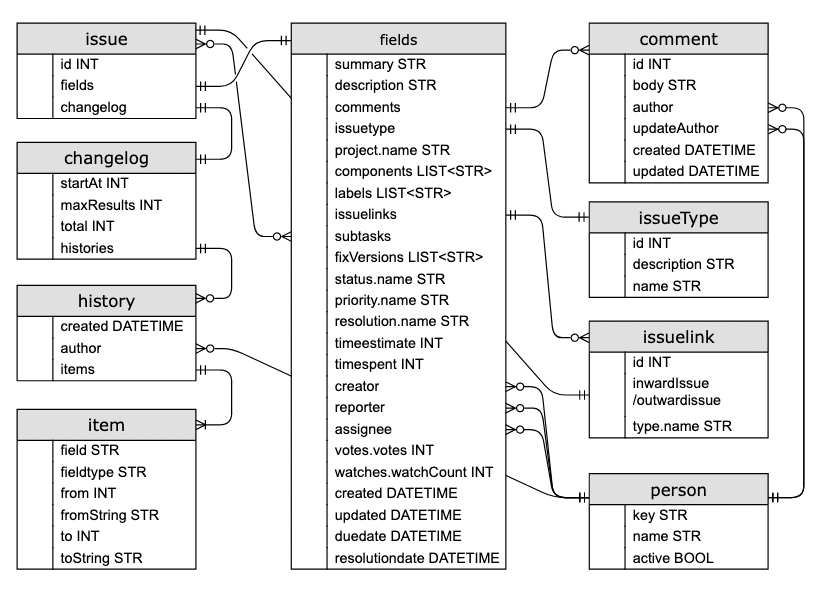
\includegraphics[width=\linewidth]{overleaf/images/ERD-jira.png}
  \caption{ERD}
\end{figure}

Figure 1 describes the entity relationship diagram (ERD) for the data set as it modelled inside the document data store MongoDB.
Due to nested values in document-oriented data stores, the ERD is a simplified depiction of the real data structure, which can include various values for the historical changes of the issues, as well as the different levels of links between issues. 
The primary documents are issues.
The two main documents nested inside each issue, are "fields" and "changelog".
The fields are are the current values of the attributes inside an issue, as described in Table 2.
The changelog are historical values of these fields, as well as some meta data, i.e. number of times changed and a date and time of the change.

\begin{table}[h!]
\caption{Description of fields in Jira issues work items.}
\centering
 \begin{tabular}{l l} 
 \hline
 \textbf{Issue field} & \textbf{Description} \\ [0.5ex] 
 \hline\hline
  & \multicolumn{1}{c}{\textbf{Issues}} \\
 summary & A brief summary of the issue. \\ 
 description & A longer, detailed description of the issue. \\
 comments & Community discussion on each issue. \\
 issuetype & The issue purpose within the organisation. \\
 project & The parent project issue belongs to. \\
 components & Project component(s) to which issue relates. \\
 labels & Label(s) to which this issue relates. \\
 issuelinks & A list of links to related issues. \\
 subtasks & Sub-issues to this issue (one level deep). \\
 fixVersions & Project version in which the issue is fixed. \\
 status & The stage the issue is at. \\
 priority & The issue importance in relation to others. \\
 resolution & A record of the issue’s resolution/closure.  \\
 timeestimate & Estimated amount of time required to resolve. \\
 timespent & Amount of time spent working on this issue. \\
 creator & The person who created the issue. \\
 reporter & The person who found/reported the issue. \\
 assignee & The person responsible to resolve the issue. \\
 votes & Number of people who want 
 this issue addressed. \\
 watches & Number of people receiving updates \\
 created & Time and date this issue was entered into Jira. \\
 updated & Time and date this issue was last edited. \\
 resolutiondate & Time and date this issue was resolved. \\
 duedate & Time and date this issue is scheduled to be \\
 & completed. \\ [2ex] 
 \hline
 \end{tabular}
\end{table}

The dataset is very extensive and complete and holds several types of data: text, datetimes, nominal and ordinal numerical data, linked network data and historical versions of all nearly every field.
The fields are a mix of singular values, lists and dictionaries.

The most important fields of the data set arguably is the enhanced mapped data of links and types.
Not only does this normalise parts of the data and reduce processing requirements, but it also adds the possibility of using these custom fields. Choetkiertikul et al. \cite{choetkiertikul2017predicting}
have showed the value of this type of data, therefore this study continues in that same direction.

\begin{table}[h!]
\caption{Dataset of Jira repositories}
\centering
 \begin{tabular}{l l l l l l} 
 \hline
   & Sum & Max & Min & Median & Std Dev \\ [0.5ex] 
 \hline\hline
 Born & - & 2016 & 2000 & TBD & TBD \\
 Issues & 2,686,282 & 1,014,926 & 1867 & 59,853 & 251,973 \\
 DIT & 485 & 122 & 1 & 18 & 31 \\
 UIT & 352 & 55 & 2 & 14 & 16 \\
 Links & 978,223 & 264,108 & 46 & 15,898 & 81,744 \\
 DLT & 180 & 23 & 6* & 10 & 6 \\
 ULT & 169 & 20 & 4 & 10 & 5 \\ 
 Ch/I & - & 30 & 3 & 12 & 6 \\
 Co/I & - & 8 & 1* & 3 & 2 \\
 UP & 1822 & 657 & 3 & 37 & 178 \\ [2ex] 
 \hline
 \end{tabular}
 \subcaption{* The two no longer available repositories do not have these values \\
 \textbf{Column names}: Documented Issue Types (DIT); Used Issue Types (UIT);
Documented Link Types (DLT); Used Link Types (ULT);
Changes per Issue (Ch/I); Comments per Issue (Co/I); Unique Projects (UP)
}
\end{table}

The data set consist of 16 public Jira repositories with a total of 1822 different project, containing 2.7 million issues. 
These issues contain historical data of 32 million changes, 9 million comments and 1 million issue links of various natures. 
Table 1 shows the complete overview of this data: the year the projects started, the number of issues, number of documented and used issue types, number of documented and used link types, number of changes per issue, number of comments per issue, and number of unique projects. 

Jira being a customizable IST explains why there are more DITs and DLTs than UIT and ULT. It is possible that some are created and are not yet or no longer used.
Custom fields are not directly usable in a possible model, due to them not being normalised.
The authors of the data set therefore enhanced the data set by mapping the links and the types to a curated number of options.
This enhancement allows for use of these custom fields, better comparison between different Jira repositories, and projects within those repositories.

The minimum number of changes on any of the nearly 2.7 million issues is 3 and the median is 12. If these are considered by the model, it would mean that the data set holds close to a magnitude more data than any of the previous researches, where nobody used this historical data.

The sprint iterations documents and boards documents retrieved from Jira hold less fields and can be seen in figure 3.
The boards are merely described in this diagram, due to each sprint needing to be contained within a board and the sprints themselves are sourced through iterating over each existing board.
The sprints do hold not hold many fields eligible to be used for analysis: the different dates allow to calculate the duration of the sprint and a difference between endDate and completeDate indicate an overrun or the administrative action of closing the sprint being done later.

\begin{figure}
\caption{ERD of the boards and sprints Jira documents}
\begin{center}
    \begin{tikzpicture}
         \pic {entity={A}{Board}{%
            id INT \\
            name STR \\
            type STR
        }};
        \pic[right=7em of A] {entity={AB}{Sprint}{%
            id INT\\
            state STR \\
            name STR \\
            originBoardId INT \\
            issues LIST<INT> \\
            startDate \\
            endDate \\
            completeDate \\
            activatedDate
        }};
        \draw[one to omany] (A.east) -- node[above]{\footnotesize is in} (AB.west);
        % {\captionof{figure}{caption 2 caption }}
    \end{tikzpicture}
\end{center}
\end{figure}


\section{Related work} 

\subsection{Agile software development} \\
Software development is known to face issues with delivering expected quality and overrun schedules and costs.\cite{dingsoyr2021managing}
Agile methodologies attempt to combat these issues through shorter delivery windows by iterative development, focusing on interaction and communication between all people involved (team members, business, stakeholders and end-users), and reducing the size of the intermediate results. 
This leads to teams being more capable to react to changing requirements and prevent waste of time and resources.\cite{cohen2004introduction}

The most widespread used Agile methodology is Scrum\cite{deemer2010scrum}. 
Following this methodology, teams work on \emph{user stories}, which are the system requirements. 
These user stories are created by the \emph{product owner} and based on the requirements as defined by the business, stakeholders, and the end-users. 
Together with the team, the product owner can \emph{refine} the stories and assign it \emph{story points}, which are arbitrary numbers that signal the amount of effort (not time) it takes to complete. 
The user stories are prioritized and stored in the \emph{product backlog} until selected. 
The team works in \emph{iterations} of work called \emph{sprints}, which are \emph{timeboxed} to usually 2-4 weeks long.
At the beginning of a sprint, the teams selects user stories from the product backlog to work on, which they intend to finish within that sprint. 
User stories can therefor never take longer than the duration of sprint; if they do, they need to be split up into smaller ones. 
User stories inside the sprint backlog do not change during the cycle. Every day there is a \emph{standup}, where each team member shares their progress on the user stories and adjust if necessary to complete the work. 
At the end of the sprint, which is \emph{timeboxed}, the team holds the \emph{review} where the outcomes are discussed and during the \emph{retrospective } they gather feedback to use during the next cycle. 
If some work is not done, it automatically rolls over to the next sprint, although this must be avoided.

Despite these benefits, a study in 2014 showed that many adaptors of the Scrum methodology (in Norway) still address theirs risks in their old, traditional approaches.\cite{siddique2014practical} Additionally, even if some problems are solved through adaptation of Scrum, new risks can possibly be introduced, such as risks in the sprint planning, risks in the code base and technologies used, an increased separation between the development and the operational work, and increased impact of technical debt\cite{kruchten2012technical}\cite{walczak2013risks}. \\

\subsection{Risks assessment and control} \\
Meerman\cite{meerman2022risk} looked at individual issues and used some of the default features of a Jira isssue: summary, description, status, type, labels, project, assignee, created, updated, resolution date, points, urgency, severity and sprint.
They made use of ensembling different models to increase performance: adaboost, bagging, random forest, gradient boost and stacking model.
The outcome was a prediction of the status: cancelled, completed or active.

For data processing, they transformed the textual data by removing capitals and stop-words and by stemming the words. 
These steps reduce the required processing power, something valuable for the larger data set used in this study.
The downside of removing stop-words, is that sequence modelling of the text is no longer possible.
The textual data was then processed to be used as input for the model through NLP techniques. Bag of words was considered, but deemed too impractical for large data sets, which is also our case.
The pre-trained text model BART was used in addition to Latent Dirichlet Allocation (LDA), which automates topic modelling and can use its output of a number of topics as input for the model.

Choetkiertikul et al.\cite{choetkiertikul2017predicting} looked at both individual issues and related issues through links, and then used collective inference to make predictions for related issues simultaniously. 
The individual issues done through the following features: discussion time, waiting time, tyep, task repetition, priority, changing of priority, no of fix versions, no of affect versions, changing of description, reporter reputation, developer's workload, percentage of delayed tasks, number of votes and number of watchers.
The related issues are done in both an explicit and implicit manner. Explicitly, every issue is linked to others and thus a relation is established. Implicitly, the authors created a model that creates its own links based on the individual issues' features.

\subsection{Machine learning models}
Todo before the next deadline on methodology

\section{Methodology}

\subsection{Machine learning models for risk assessment}\\
Based on the EDA and related work, this study will use the following methods and achieve the following goals:

* pre-process the textual data in the same manner as Meerman 

* use ensembling as well, due to the variance and size of the input data

* make use of the NLP methods as done by Meerman, to reduce required processing power.

* our model will make a prediction on status (at the end of a sprint), number of changes of the field sprint, duedate, resolutiondate.

\subsection{Methods to share risk control}\\
Besides having a model that can assess the risk, it also needs to share which specific elements are causing the risk. These need to be reported to the team.

The team should be able to adjust the user stories added to a sprint and immediately receive feedback on the risk score of the current sprint planning.

Stretch ambition might be to automatically suggest which user stories from the top of the product backlog should be added to a sprint. For this to become a reality, team velocity based on story points should be present, possibly from other models.

A platform to offer such a service could be through Atlassian Marketplace, where various Jira Apps are offered to be used inside the planning software.


\section{Risk Assessment}\\
A few potential risks can be identified regarding the research as described in this thesis design. In this section, these risks will be discussed, and if needed, a back-up plan will be formulated.

While finding data sets including product backlogs with user stories is relatively simple, it will only be useful if it includes sprint data. This can be resolved by using data sets that have not yet been processed to remove this information.

The found data sets from different planning software might require different types of processing. Fortunately it is already labeled, so it should comprise mostly of cleaning the data sets. Another benefit is the availability of good scripting skills and available budget to outsource it.

Besides different models in which the data resides, entries in the data sets can widely vary between organisations and even between teams of the same organisation. This might introduce a risk of the model only being able to properly train on its own data set. This could possibly be turned around into an advantage, because the moment this occurs and is resolved, it should mean that the data model is applicable to new data sets as well.

For this study, I am dependent on previous study to supply the ML model. In the worst case scenario, I should be able to fall back to more basic models found in literature.

There is always the risk of the ML model accuracy not being significant. If this is the case, the main focus of the project should switch from risk assessment to risk control or vise versa.


\section{Project Planning}

\emph{Figure 1} below shows an overview of the week-by-week planning for the thesis project. Yellow bars are the deadlines weeks set by UvA as feedback moments. Calendar week 4 is Monday 14 of February, week 26 is Monday 27 of June. 

\begin{figure}[h]
  \centering
  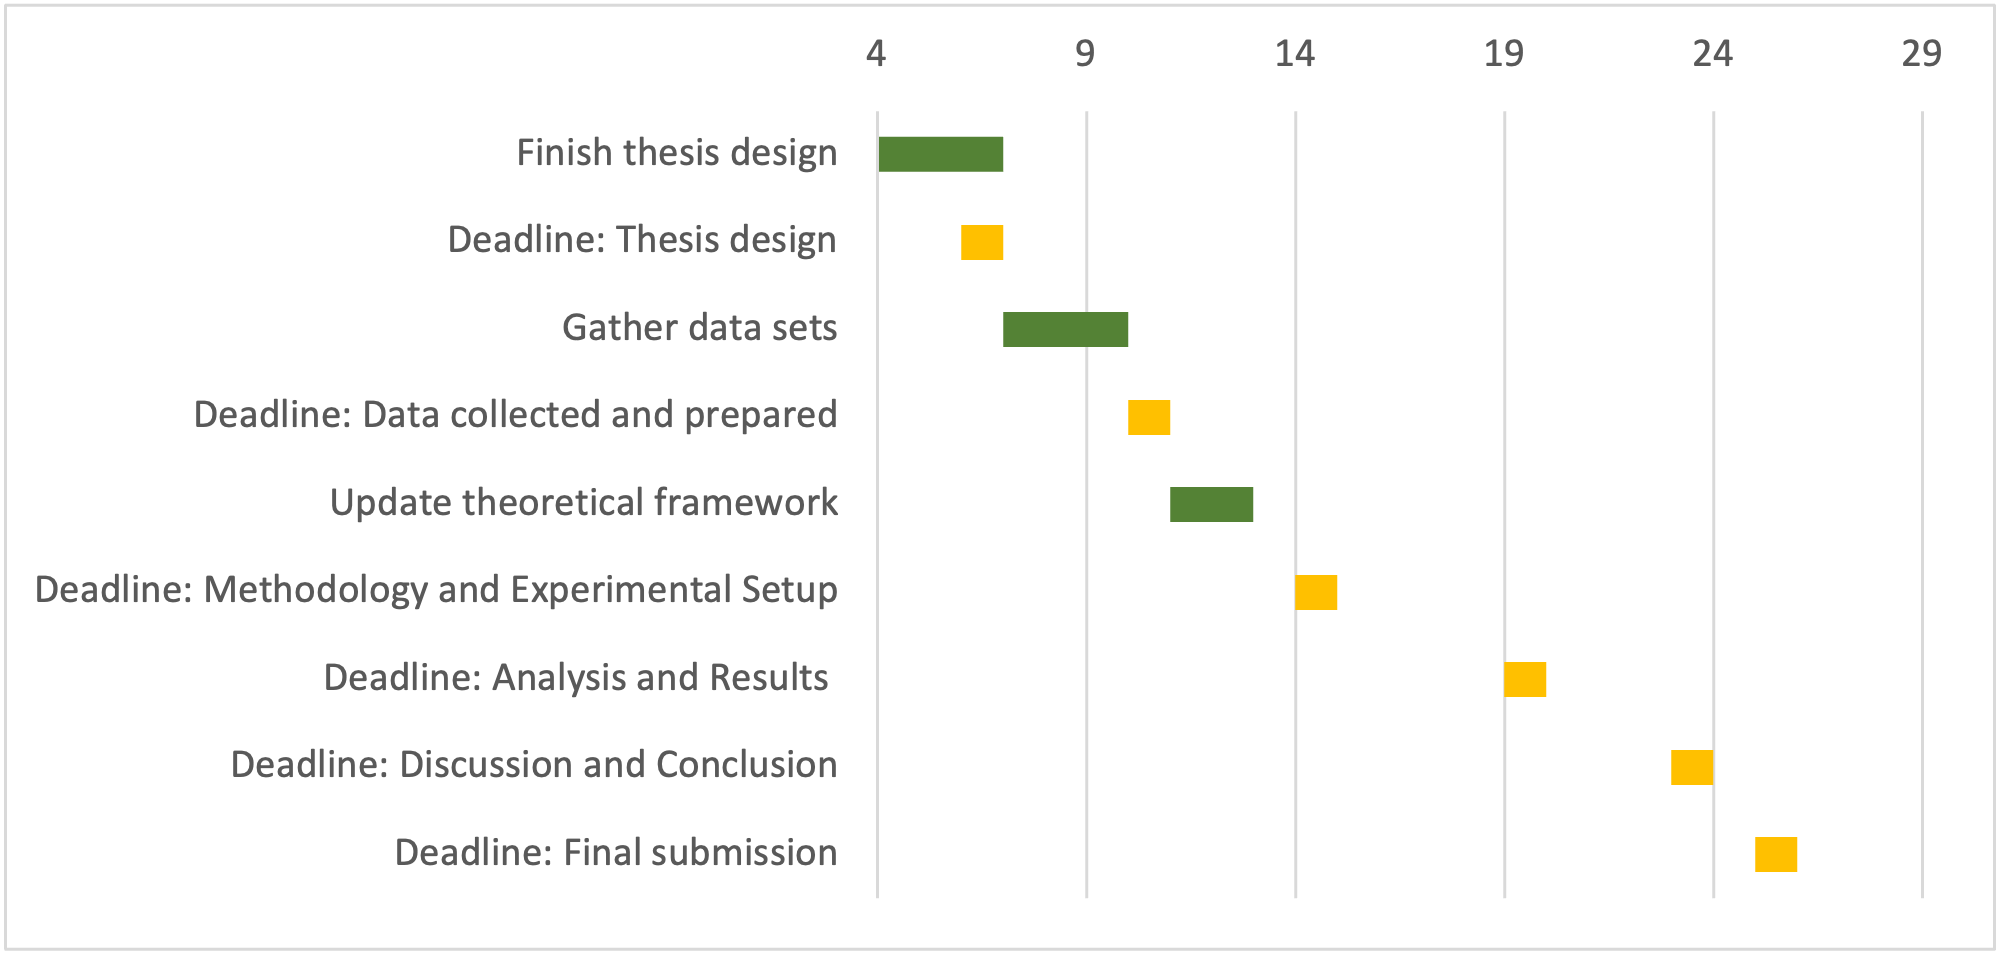
\includegraphics[width=\linewidth]{gantt-planning}
  \caption{Gantt chart on planning per calendar week.}
\end{figure}

\section{Future work}
Look at project level instead of jira-repo level.

%%
%% The acknowledgments section is defined using the "acks" environment
%% (and NOT an unnumbered section). This ensures the proper
%% identification of the section in the article metadata, and the
%% consistent spelling of the heading.


%%
%% The next two lines define the bibliography style to be used, and
%% the bibliography file.
\bibliographystyle{ACM-Reference-Format}
\bibliography{sample-base}

%%
%% If your work has an appendix, this is the place to put it.
\appendix


\end{document}
\endinput
%%
%% End of file `sample-lualatex.tex'.
